\documentclass[11pt,a4paper]{article}

\usepackage[a4paper,margin=1in]{geometry}
\usepackage{multicol}
\usepackage{enumitem}
\usepackage{fancyhdr}
\usepackage{setspace}
\usepackage{amsmath}
\usepackage{float}
\usepackage{graphicx}
\usepackage{gvv}
\usepackage{gvv-book}
\usepackage{listings}
\lstset{frame=single, breaklines=true, columns=fullflexible}
\usepackage{caption}
\usepackage[normalem]{ulem}

\pagestyle{fancy}
\fancyhf{}
\fancyhead[L]{GATE 2024}
\fancyhead[C]{\textbf{General Aptitude}}
\fancyfoot[C]{\thepage}

\setlength{\parindent}{0pt}
\setlength{\parskip}{2pt}
\begin{document}
\title{GATE 2022 - General Aptitude}
\author{ee25btech11005-Aditya Mishra}
\maketitle

{\let\newpage\relax\maketitle}

\renewcommand{\thefigure}{\theenumi}
\renewcommand{\thetable}{\theenumi}
\setlength{\intextsep}{10pt} 

\begin{enumerate}

\item The \rule{2cm}{0.4pt} is too high for it to be considered \rule{2cm}{0.4pt}  

\begin{enumerate}
\begin{multicols}{4}
\item fair / fare
\item faer / fair
\item fare / fare
\item fare / fair
\end{multicols}
\end{enumerate}

\hfill{\brak{\text{GATE CS 2022}}}

\item A function $y(x)$ is defined in the interval $\brak{0,1}$ on the $x$-axis as  

\[
y(x) = 
\begin{cases} 
2 & 0 \leq x < \tfrac{1}{3} \\
3 & \tfrac{1}{3} \leq x < \tfrac{3}{4} \\
1 & \tfrac{3}{4} \leq x \leq 1
\end{cases}
\]

Which one of the following is the area under the curve for the interval $\brak{0,1}$ on the $x$-axis?  

\begin{enumerate}
\begin{multicols}{4}
\item $\tfrac{5}{6}$
\item $\tfrac{6}{5}$
\item $\tfrac{13}{6}$
\item $\tfrac{6}{13}$
\end{multicols}
\end{enumerate}

\hfill{\brak{\text{GATE CS 2022}}}

\item Let $r$ be a root of the equation $x^2 + 2x + 6 = 0$. Then the value of the expression \brak{r+2}\brak{r+3}\brak{r+4}\brak{r+5} is  

\begin{enumerate}
\begin{multicols}{4}
\item 51
\item $-51$
\item 126
\item $-126$
\end{multicols}
\end{enumerate}

\hfill{\brak{\text{GATE CS 2022}}}

\item Given below are four statements.  

Statement 1: All students are inquisitive.  

Statement 2: Some students are inquisitive.  

Statement 3: No student is inquisitive.  

Statement 4: Some students are not inquisitive.  

From the given four statements, find the two statements that CANNOT BE TRUE simultaneously, assuming that there is at least one student in the class.  

\begin{enumerate}
\begin{multicols}{2}
\item Statement 1 and Statement 3
\item Statement 1 and Statement 2
\item Statement 2 and Statement 4
\item Statement 3 and Statement 4
\end{multicols}
\end{enumerate}

\hfill{\brak{\text{GATE CS 2022}}}

\item A palindrome is a word that reads the same forwards and backwards. In a game of words, a player has the following two plates painted with letters.  
\begin{figure}[H]
\centering
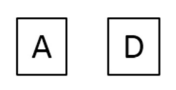
\includegraphics[width=0.4\columnwidth]{figs/q5-1.png}
\caption{Fig: q5}
\label{fig:q5}
\end{figure}

From the additional plates given in the options, which one of the combinations of additional plates would allow the player to construct a five-letter palindrome. The player should use all the five plates exactly once. The plates can be rotated in their plane.  

\begin{enumerate}
\item 
\begin{figure}[H]
\centering
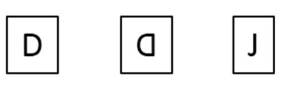
\includegraphics[width=0.4\columnwidth]{figs/q5-2.png}
\caption{Option1}
\label{fig:q5}
\end{figure}
\item 
\begin{figure}[H]
\centering
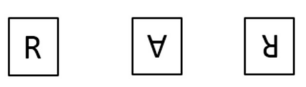
\includegraphics[width=0.4\columnwidth]{figs/q5-3.png}
\caption{Option2}
\label{fig:q5}
\end{figure}
\item 
\begin{figure}[H]
\centering
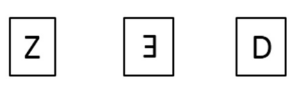
\includegraphics[width=0.4\columnwidth]{figs/q5-4.png}
\caption{Option3}
\label{fig:q5}
\end{figure}
\item 
\begin{figure}[H]
\centering
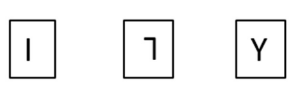
\includegraphics[width=0.4\columnwidth]{figs/q5-5.png}
\caption{Option4}
\label{fig:q5}
\end{figure}
\end{enumerate}

\hfill{\brak{\text{GATE CS 2022}}}

\item Some people believe that ``what gets measured, improves''. Some others believe that ``what gets measured, gets gamed''. One possible reason for the difference in the beliefs is the work culture in organizations. In organizations with good work culture, metrics help improve outcomes. However, the same metrics are counterproductive in organizations with poor work culture.  

Which one of the following is the CORRECT logical inference based on the information in the above passage?  

\begin{enumerate}
\item Metrics are useful in organizations with poor work culture
\item Metrics are useful in organizations with good work culture
\item Metrics are always counterproductive in organizations with good work culture
\item Metrics are never useful in organizations with good work culture
\end{enumerate}

\hfill{\brak{\text{GATE CS 2022}}}

\item In a recently conducted national entrance test, boys constituted 65\% of those who appeared for the test. Girls constituted the remaining candidates and they accounted for 60\% of the qualified candidates.  

Which one of the following is the correct logical inference based on the information provided in the above passage?  

\begin{enumerate}
\item Equal number of boys and girls qualified
\item Equal number of boys and girls appeared for the test
\item The number of boys who appeared for the test is less than the number of girls who appeared
\item The number of boys who qualified the test is less than the number of girls who qualified
\end{enumerate}

\hfill{\brak{\text{GATE CS 2022}}}

\item A box contains five balls of same size and shape. Three of them are green coloured balls and two of them are orange coloured balls. Balls are drawn from the box one at a time. If a green ball is drawn, it is not replaced. If an orange ball is drawn, it is replaced with another orange ball.  

First ball is drawn. What is the probability of getting an orange ball in the next draw?  

\begin{enumerate}
\begin{multicols}{4}
\item $\tfrac{1}{2}$
\item $\tfrac{8}{25}$
\item $\tfrac{19}{50}$
\item $\tfrac{23}{50}$
\end{multicols}
\end{enumerate}

\hfill{\brak{\text{GATE CS 2022}}}

\item The corners and mid-points of the sides of a triangle are named using the distinct letters P, Q, R, S, T and U, but not necessarily in the same order. Consider the following statements:  

\begin{itemize}
\item The line joining P and R is parallel to the line joining Q and S.  
\item P is placed on the side opposite to the corner T.  
\item S and U cannot be placed on the same side.  
\end{itemize}

Which one of the following statements is correct based on the above information?  

\begin{enumerate}
\begin{multicols}{2}
\item P cannot be placed at a corner
\item S cannot be placed at a corner
\item U cannot be placed at a mid-point
\item R cannot be placed at a corner
\end{multicols}
\end{enumerate}

\hfill{\brak{\text{GATE CS 2022}}}

\item A plot of land must be divided between four families. They want their individual plots to be similar in shape, not necessarily equal in area. The land has equally spaced poles, marked as dots in the below figure. Two ropes, $R_1$ and $R_2$, are already present and cannot be moved.  

What is the least number of additional straight ropes needed to create the desired plots? A single rope can pass through three poles that are aligned in a straight line. \begin{figure}[H]
\centering
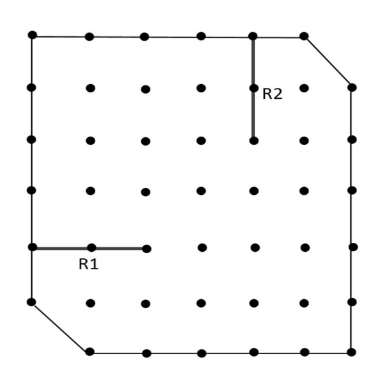
\includegraphics[width=0.8\columnwidth]{figs/q10.png}
\caption{Fig}
\label{fig:q10}
\end{figure}

\begin{enumerate}
\begin{multicols}{4}
\item 2
\item 4
\item 5
\item 3
\end{multicols}
\end{enumerate}

\hfill{\brak{\text{GATE CS 2022}}}

\item Which one of the following statements is TRUE for all positive functions $f(n)$?  

\begin{enumerate}
\item $f(n)^2 = \theta(f(n^2))$ when $f(n)$ is a polynomial
\item $f(n)^2 = o(f(n^2))$
\item $f(n)^2 = O(f(n^2))$ when $f(n)$ is an exponential function
\item $f(n)^2 = \Omega(f(n^2))$
\end{enumerate}

\hfill{\brak{\text{GATE CS 2022}}}

\item Which one of the following regular expressions correctly represents the language of the finite automaton given below?  
\begin{figure}[H]
\centering
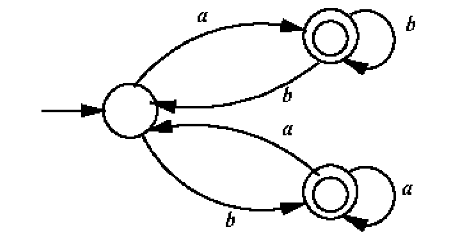
\includegraphics[width=0.8\columnwidth]{figs/q12.png}
\caption{Figure for question}
\label{fig:q12}
\end{figure}
\begin{enumerate}
\item $ab^* bab^* ba^* aba^*$
\item $(ab^* b ab^* ba^* a ba^*)^*$
\item $(ab^* b ba^* a^* b)^*$
\item $(ba^* a ab^* b ab^* ba^*)^*$
\end{enumerate}

\hfill{\brak{\text{GATE CS 2022}}}

\item Which one of the following statements is TRUE?  

\begin{enumerate}
\item The LALR(1) parser for a grammar G cannot have reduce-reduce conflict if the LR(1) parser for G does not have reduce-reduce conflict
\item Symbol table is accessed only during the lexical analysis phase
\item Data flow analysis is necessary for run-time memory management
\item LR(1) parsing is sufficient for deterministic context-free languages
\end{enumerate}

\hfill{\brak{\text{GATE CS 2022}}}

\item In a relational data model, which one of the following statements is TRUE?  

\begin{enumerate}
\item A relation with only two attributes is always in BCNF
\item If all attributes of a relation are prime attributes, then the relation is in BCNF
\item Every relation has at least one non-prime attribute
\item BCNF decompositions preserve functional dependencies
\end{enumerate}

\hfill{\brak{\text{GATE CS 2022}}}

\item Consider the problem of reversing a singly linked list. To take an example, given the linked list below,  
\begin{figure}[H]
\centering
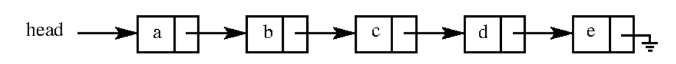
\includegraphics[width=0.8\columnwidth]{figs/q15-1.png}
\caption{Link 1}
\label{fig:q15}
\end{figure}
the reversed linked list should look like  
\begin{figure}[H]
\centering
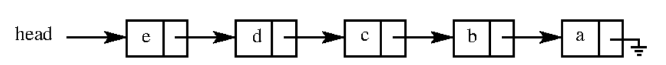
\includegraphics[width=0.8\columnwidth]{figs/q15-2.png}
\caption{Link 2}
\label{fig:q15}
\end{figure}
Which one of the following statements is TRUE about the time complexity of algorithms that solve the above problem in $O(1)$ space?  

\begin{enumerate}
\begin{multicols}{2}
\item The best algorithm for the problem takes $\theta(n)$ time in the worst case
\item The best algorithm for the problem takes $\theta(n \log n)$ time in the worst case
\item The best algorithm for the problem takes $\theta(n^2)$ time in the worst case
\item It is not possible to reverse a singly linked list in $O(1)$ space
\end{multicols}
\end{enumerate}

\hfill{\brak{\text{GATE CS 2022}}}

\item Suppose we are given $n$ keys, $m$ hash table slots, and two simple uniform hash functions $h_1$ and $h_2$. Further suppose our hashing scheme uses $h_1$ for the odd keys and $h_2$ for the even keys. What is the expected number of keys in a slot?  

\begin{enumerate}
\begin{multicols}{4}
\item $\tfrac{m}{n}$
\item $\tfrac{n}{m}$
\item $\tfrac{2n}{m}$
\item $\tfrac{n}{2m}$
\end{multicols}
\end{enumerate}

\hfill{\brak{\text{GATE CS 2022}}}

\item Which one of the following facilitates transfer of bulk data from hard disk to main memory with the highest throughput?  

\begin{enumerate}
\begin{multicols}{2}
\item DMA based I/O transfer
\item Interrupt driven I/O transfer
\item Polling based I/O transfer
\item Programmed I/O transfer
\end{multicols}
\end{enumerate}

\hfill{\brak{\text{GATE CS 2022}}}

\item Let R1 and R2 be two 4-bit registers that store numbers in 2’s complement form. For the operation R1+R2, which one of the following values of R1 and R2 gives an arithmetic overflow?  

\begin{enumerate}
\begin{multicols}{2}
\item R1 = 1011 and R2 = 1110
\item R1 = 1100 and R2 = 1010
\item R1 = 0011 and R2 = 0100
\item R1 = 1001 and R2 = 1111
\end{multicols}
\end{enumerate}

\hfill{\brak{\text{GATE CS 2022}}}

\item Consider the following threads, T1, T2, and T3 executing on a single processor, synchronized using three binary semaphore variables, S1, S2, and S3, operated upon using standard wait() and signal(). The threads can be context switched in any order and at any time.  
\begin{table}[H]
\centering
\begin{tabular}{|c|c|c|}
\hline
T1 & T2 & T3 \\
\hline
\begin{minipage}{0.28\linewidth}
\begin{verbatim}
while(true){
 wait(S3);
 print("C");
 signal(S2); }
\end{verbatim}
\end{minipage}
&
\begin{minipage}{0.28\linewidth}
\begin{verbatim}
while(true){
 wait(S1);
 print("B");
 signal(S3); }
\end{verbatim}
\end{minipage}
&
\begin{minipage}{0.28\linewidth}
\begin{verbatim}
while(true){
 wait(S2);
 print("A");
 signal(S1); }
\end{verbatim}
\end{minipage}
\\
\hline
\end{tabular}
\caption*{}
\label{tab:q19}
\end{table}

Which initialization of the semaphores would print the sequence BCABCABCA….?  

\begin{enumerate}
\begin{multicols}{2}
\item S1 = 1; S2 = 1; S3 = 1
\item S1 = 1; S2 = 1; S3 = 0
\item S1 = 1; S2 = 0; S3 = 0
\item S1 = 0; S2 = 1; S3 = 1
\end{multicols}
\end{enumerate}

\hfill{\brak{\text{GATE CS 2022}}}

\item Consider the following two statements with respect to the matrices $A_{m \times n}, B_{n \times m}, C_{n \times n}, D_{n \times n}$.  

Statement 1: $\text{tr}(AB) = \text{tr}(BA)$  

Statement 2: $\text{tr}(CD) = \text{tr}(DC)$  

Which one of the following holds?  

\begin{enumerate}
\item Statement 1 is correct and Statement 2 is wrong
\item Statement 1 is wrong and Statement 2 is correct
\item Both Statement 1 and Statement 2 are correct
\item Both Statement 1 and Statement 2 are wrong
\end{enumerate}

\hfill{\brak{\text{GATE CS 2022}}}

\item What is printed by the following ANSI C program?  

\begin{verbatim}
#include<stdio.h>
int main(int argc, char *argv[]){
 int x = 1, z[2] = {10,11};
 int *p = NULL;
 p = &x;
 *p = 10;
 p = &z[1];
 *(&z[0]+1) += 3;
 printf("%d, %d, %d\n", x, z[0], z[1]);
 return 0;
}
\end{verbatim}

\begin{enumerate}
\begin{multicols}{2}
\item 1, 10, 11
\item 1, 10, 14
\item 10, 14, 11
\item 10, 10, 14
\end{multicols}
\end{enumerate}

\hfill{\brak{\text{GATE CS 2022}}}

\item Consider an enterprise network with two Ethernet segments, a web server and a firewall, connected via three routers. What is the number of subnets inside the enterprise network?  
\begin{figure}[H]
\centering
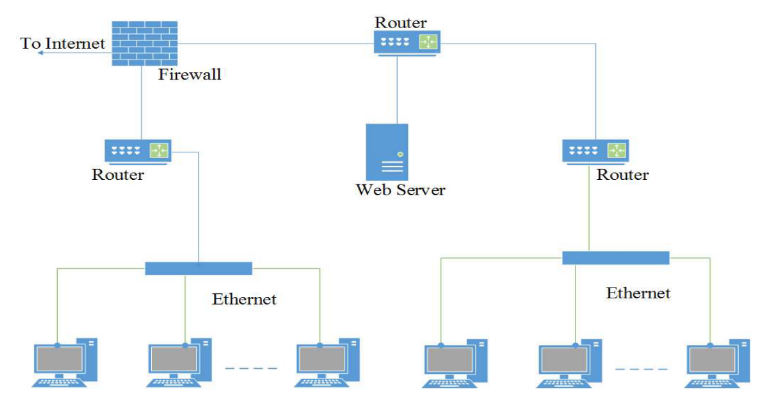
\includegraphics[width=0.8\columnwidth]{figs/q22.png}
\caption{Figure for Q22}
\label{fig:q22}
\end{figure}
\begin{enumerate}
\begin{multicols}{4}
\item 3
\item 12
\item 6
\item 8
\end{multicols}
\end{enumerate}

\hfill{\brak{\text{GATE CS 2022}}}

\item Which of the following statements is/are TRUE?  

\begin{enumerate}
\item Every subset of a recursively enumerable language is recursive
\item If a language L and its complement $\bar{L}$ are both recursively enumerable, then L must be recursive
\item Complement of a context-free language must be recursive
\item If $L_1$ and $L_2$ are regular, then $L_1 \cap L_2$ must be deterministic context-free
\end{enumerate}

\hfill{\brak{\text{GATE CS 2022}}}

\item Let WB and WT be two set associative cache organizations that use LRU algorithm for cache block replacement. WB is a write back cache and WT is a write through cache. Which of the following statements is/are FALSE?  

\begin{enumerate}
\item Each cache block in WB and WT has a dirty bit
\item Every write hit in WB leads to a data transfer from cache to main memory
\item Eviction of a block from WT will not lead to data transfer from cache to main memory
\item A read miss in WB will never lead to eviction of a dirty block from WB
\end{enumerate}

\hfill{\brak{\text{GATE CS 2022}}}

\item Consider the following three relations in a relational database.  

Employee(eId, Name), Brand(bId, bName), Own(eId, bId)  

Which of the following relational algebra expressions return the set of eIds who own all the brands?  

\begin{enumerate}
\item $\pi_{eId}\brak{ \pi_{eId,bId}Own \div \pi_{bId}Brand }$
\item $\pi_{eId}\brak{ \pi_{eId}Own - \pi_{eId}\brak{ \pi_{eId,bId}Own \times \pi_{bId}Brand - \pi_{eId,bId}Own } }$
\item $\pi_{eId}\brak{ \pi_{eId,bId}Own \div \pi_{bId}Own }$
\item $\pi_{eId}\brak{ \brak{\pi_{eId,bId}Own \times \pi_{bId}Own} \div \pi_{bId}Brand }$
\end{enumerate}

\hfill{\brak{\text{GATE CS 2022}}}

\item Which of the following statements is/are TRUE with respect to deadlocks?  

\begin{enumerate}
\item Circular wait is a necessary condition for the formation of deadlock
\item In a system where each resource has more than one instance, a cycle in its wait-for graph indicates the presence of a deadlock
\item If the current allocation of resources to processes leads the system to unsafe state, then deadlock will necessarily occur
\item In the resource-allocation graph of a system, if every edge is an assignment edge, then the system is not in deadlock state
\end{enumerate}

\hfill{\brak{\text{GATE CS 2022}}}

\item Which of the following statements is/are TRUE for a group $G$?  

\begin{enumerate}
\item If for all $x,y \in G$, $(xy)^2 = x^2y^2$, then G is commutative
\item If for all $x \in G$, $x^2=1$, then G is commutative
\item If the order of G is 2, then G is commutative
\item If G is commutative, then a subgroup of G need not be commutative
\end{enumerate}

\hfill{\brak{\text{GATE CS 2022}}}

\item Suppose a binary search tree with 1000 distinct elements is also a complete binary tree. The tree is stored using the array representation of binary heap trees. Assuming that the array indices start with 0, the 3rd largest element of the tree is stored at index \rule{2cm}{0.4pt}  

\hfill{\brak{\text{GATE CS 2022}}}

\item Consider the augmented grammar with $\{id,+,*,\brak{,},\}$ as the set of terminals.  

\[
S' \to S, \quad S \to S+R \mid R, \quad R \to R*P \mid P, \quad P \to (S) \mid id
\]  

If $I_0 = \{ [S' \to \cdot S], [S \to \cdot S+R] \}$, then $closure(goto(I_0,+))$ contains exactly \rule{2cm}{0.4pt} items.  

\hfill{\brak{\text{GATE CS 2022}}}

\item Consider a simple undirected graph of 10 vertices. If the graph is disconnected, then the maximum number of edges it can have is \rule{2cm}{0.4pt}  

\hfill{\brak{\text{GATE CS 2022}}}

\item Consider a relation $R(A,B,C,D,E)$ with the following three functional dependencies:  

$AB \to C, \; BC \to D, \; C \to E$.  

The number of superkeys in the relation R is \rule{2cm}{0.4pt}  

\hfill{\brak{\text{GATE CS 2022}}}

\item The number of arrangements of six identical balls in three identical bins is \rule{2cm}{0.4pt}  

\hfill{\brak{\text{GATE CS 2022}}}

\item A cache memory that has a hit rate of 0.8 has an access latency 10 ns and miss penalty 100 ns. An optimization is done on the cache to reduce the miss rate. However, the optimization results in an increase of cache access latency to 15 ns, whereas the miss penalty is not affected. The minimum hit rate (rounded off to two decimal places) needed after the optimization such that it should not increase the average memory access time is \rule{2cm}{0.4pt}  

\hfill{\brak{\text{GATE CS 2022}}}

\item The value of the following limit is \rule{2cm}{0.4pt}  

\[
\lim_{x \to 0+} \frac{\sqrt{x}}{1 - e^{2\sqrt{x}}}
\]

\hfill{\brak{\text{GATE CS 2022}}}

\item Consider the resolution of the domain name www.gate.org.in by a DNS resolver. Assume that no resource records are cached anywhere across the DNS servers and that iterative query mechanism is used in the resolution. The number of DNS query-response pairs involved in completely resolving the domain name is \rule{2cm}{0.4pt}  

\hfill{\brak{\text{GATE CS 2022}}}


\item Which one of the following is the closed form for the generating function of the sequence $\{a_n\}_{n \geq 0}$ defined below?  

\[
a_n = \begin{cases} 
1, & n \text{ is odd} \\
1, & \text{otherwise}
\end{cases}
\]

\begin{enumerate}
\item $\dfrac{1+x}{(1-x)(1-x^2)}$
\item $\dfrac{1-3x+x^2}{(1-x)(1-x^2)}$
\item $\dfrac{1+x^2}{(1-x)(1-x^2)}$
\item $\dfrac{1}{(1-x)(1+x)}$
\end{enumerate}

\hfill{\brak{\text{GATE CS 2022}}}

\item Consider a simple undirected unweighted graph with at least three vertices. If $A$ is the adjacency matrix of the graph, then the number of 3-cycles in the graph is given by the trace of  

\begin{enumerate}
\begin{multicols}{2}
\item $A^3$
\item $A^3/2$
\item $A^3/3$
\item $A^3/6$
\end{multicols}
\end{enumerate}

\hfill{\brak{\text{GATE CS 2022}}}

\item Which one of the following statements is FALSE?  

\begin{enumerate}
\item The TLB performs an associative search in parallel on all its valid entries using page number of incoming virtual address
\item If the virtual address of a word given by CPU has a TLB hit, but the subsequent search for the word results in a cache miss, then the word will always be present in the main memory
\item The memory access time using a given inverted page table is always same for all incoming virtual addresses
\item In a system that uses hashed page tables, if two distinct virtual addresses $V_1$ and $V_2$ map to the same value while hashing, then the memory access time of these addresses will not be the same
\end{enumerate}

\hfill{\brak{\text{GATE CS 2022}}}

\item Let $R_i(z)$ and $W_i(z)$ denote read and write operations on a data element $z$ by a transaction $T_i$, respectively. Consider the schedule S with four transactions.  

$S: R_4(x)\;R_2(x)\;R_3(x)\;R_1(y)\;W_1(y)\;W_2(x)\;W_3(y)\;R_4(y)$  

Which one of the following serial schedules is conflict equivalent to S?  

\begin{enumerate}
\item $T_4 \to T_2 \to T_3 \to T_1$
\item $T_2 \to T_1 \to T_3 \to T_4$
\item $T_3 \to T_2 \to T_4 \to T_1$
\item $T_1 \to T_3 \to T_2 \to T_4$
\end{enumerate}

\hfill{\brak{\text{GATE CS 2022}}}

\item Consider a digital display system (DDS) that displays the contents of register X. A 16-bit code word is used to load a word in X, either from S or from R. S is a 1024-word memory segment and R is a 32-word register file. Based on the value of mode bit M, T selects an input word to load in X. P and Q interface with the corresponding bits in the code word to choose the addressed word. Which one of the following represents the functionality of P, Q, and T?  
\begin{figure}[H]
\centering
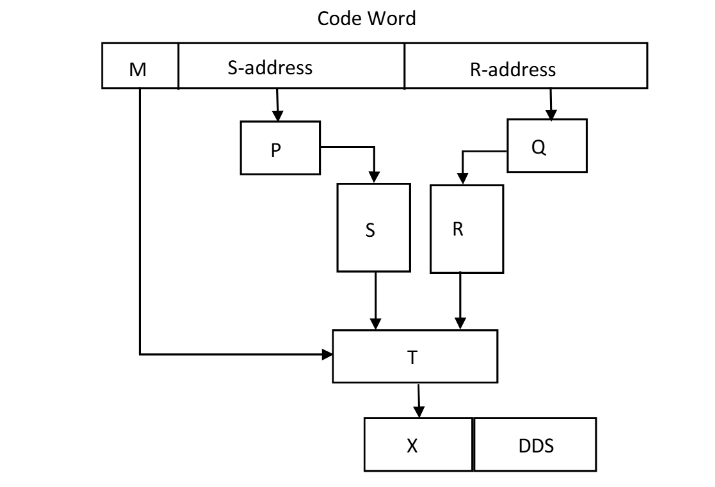
\includegraphics[width=0.8\columnwidth]{figs/q40.png}
\caption{Figure for Q40}
\label{fig:q40}
\end{figure}
\begin{enumerate}
\item P is 10:1 multiplexer; Q is 5:1 multiplexer; T is 2:1 multiplexer
\item P is $10:2^{10}$ decoder; Q is $5:2^5$ decoder; T is 2:1 encoder
\item P is $10:2^{10}$ decoder; Q is $5:2^5$ decoder; T is 2:1 multiplexer
\item P is 1:10 de-multiplexer; Q is 1:5 de-multiplexer; T is 2:1 multiplexer
\end{enumerate}

\hfill{\brak{\text{GATE CS 2022}}}

\item Consider three floating point numbers A, B and C stored in registers RA, RB and RC, respectively as per IEEE-754 single precision floating point format. The 32-bit content stored in these registers (in hexadecimal form) are as follows:  

\begin{table}[h!]
\centering
\begin{tabular}{|c|c|c|}
\hline
RA = 0xC1400000 & RB = 0x42100000 & RC = 0x41400000 \\
\hline
\end{tabular}
\caption*{}
\label{tab:q41}
\end{table} 

Which one of the following is FALSE?  

\begin{enumerate}
\item $A+C=0$
\item $C=A+B$
\item $3B=C$
\item $(B-C) > 0$
\end{enumerate}

\hfill{\brak{\text{GATE CS 2022}}}

\item Consider four processes P, Q, R, and S scheduled on a CPU as per round robin algorithm with a time quantum of 4 units. The processes arrive in the order P, Q, R, S, all at time t=0. There is exactly one context switch from S to Q, exactly one context switch from R to Q, and exactly two context switches from Q to R. There is no context switch from S to P. Switching to a ready process after the termination of another process is also considered a context switch. Which one of the following is NOT possible as CPU burst time (in time units) of these processes?  

\begin{enumerate}
\item P=4, Q=10, R=6, S=2
\item P=2, Q=9, R=5, S=1
\item P=4, Q=12, R=5, S=4
\item P=3, Q=7, R=7, S=3
\end{enumerate}

\hfill{\brak{\text{GATE CS 2022}}}

\item What is printed by the following ANSI C program?  

\begin{verbatim}
#include<stdio.h>
int main(int argc, char *argv[]){
 int a[3][3][3] = {
  {1,2,3,4,5,6,7,8,9},
  {10,11,12,13,14,15,16,17,18},
  {19,20,21,22,23,24,25,26,27}};
 int i=0,j=0,k=0;
 for(i=0;i<3;i++){
  for(k=0;k<3;k++)
   printf("%d ", a[i][j][k]);
  printf("\n");
 }
 return 0;
}
\end{verbatim}

\begin{enumerate}
\item 1 2 3; 10 11 12; 19 20 21
\item 1 4 7; 10 13 16; 19 22 25
\item 1 2 3; 4 5 6; 7 8 9
\item 1 2 3; 13 14 15; 25 26 27
\end{enumerate}

\hfill{\brak{\text{GATE CS 2022}}}

\item What is printed by the following ANSI C program?  

\begin{verbatim}
#include<stdio.h>
int main(int argc, char *argv[]){
 char a='P';
 char b='x';
 char c=(a & b)+'*';
 char d=(a | b) - '-';
 char e=(a ^ b) + '+';
 printf("%c %c %c\n", c, d, e);
 return 0;
}
\end{verbatim}

ASCII encoding for relevant characters is given.

\begin{tabular}{|c|c|c|c|c|}
\hline
A & B & C & $\cdots$ & Z \\
\hline
65 & 66 & 67 & $\cdots$ & 90 \\
\hline
\end{tabular}
\begin{tabular}{|c|c|c|c|c|}
\hline
a & b & c & $\cdots$ & z \\
\hline
97 & 98 & 99 & $\cdots$ & 122 \\
\hline
\end{tabular}
\begin{center}
\begin{tabular}{|c|c|c|}
\hline
* & + & - \\
\hline
42 & 43 & 45 \\
\hline
\end{tabular}
\end{center}
\begin{enumerate}
\begin{multicols}{2}
\item z K S
\item 122 75 83
\item * - +
\item P x +
\end{multicols}
\end{enumerate}

\hfill{\brak{\text{GATE CS 2022}}}

\item Consider solving the following system of simultaneous equations using LU decomposition.  

\[
x_1+2x_2-3x_3=4,\quad 2x_1+3x_2-7x_3=5,\quad x_1+2x_2-2x_3=7
\]

Which one of the following is the correct combination of values for $L_{32}, U_{33}, x_1$?  

\begin{enumerate}
\item $L_{32}=\tfrac{1}{2}, U_{33}=-1, x_1=-1$
\item $L_{32}=1, U_{33}=2, x_1=-1$
\item $L_{32}=-\tfrac{1}{2}, U_{33}=2, x_1=0$
\item $L_{32}=-\tfrac{1}{2}, U_{33}=-\tfrac{1}{2}, x_1=0$
\end{enumerate}

\hfill{\brak{\text{GATE CS 2022}}}

\item Which of the following is/are undecidable?  

\begin{enumerate}
\item Given two Turing machines $M_1$ and $M_2$, decide if $L(M_1)=L(M_2)$
\item Given a Turing machine $M$, decide if $L(M)$ is regular
\item Given a Turing machine $M$, decide if $M$ accepts all strings
\item Given a Turing machine $M$, decide if $M$ takes more than $10^{73}$ steps on every string
\end{enumerate}

\hfill{\brak{\text{GATE CS 2022}}}

\item Consider the following languages:  

$L_1=\{a^nwa^n \mid w \in \{a,b\}^*\}$  

$L_2=\{wxw^R \mid w,x \in \{a,b\}^*, |w|,|x|>0\}$  

Which of the following is/are TRUE?  

\begin{enumerate}
\item $L_1$ and $L_2$ are regular
\item $L_1$ and $L_2$ are context-free
\item $L_1$ is regular and $L_2$ is context-free
\item $L_1$ and $L_2$ are context-free but not regular
\end{enumerate}

\hfill{\brak{\text{GATE CS 2022}}}

\item Consider the following languages:  

$L_1=\{ww \mid w \in \{a,b\}^*\}$  

$L_2=\{a^n b^m c^n \mid m,n \geq 0\}$  

$L_3=\{a^m b^n c^n \mid m,n \geq 0\}$  

Which of the following statements is/are FALSE?  

\begin{enumerate}
\item $L_1$ is not context-free but $L_2$ and $L_3$ are deterministic context-free
\item Neither $L_1$ nor $L_2$ is context-free
\item $L_2,L_3$ and $L_2 \cap L_3$ all are context-free
\item Neither $L_1$ nor its complement is context-free
\end{enumerate}

\hfill{\brak{\text{GATE CS 2022}}}

\item Consider a simple undirected weighted graph $G$, all of whose edge weights are distinct. Which of the following statements about the minimum spanning trees of $G$ is/are TRUE?  

\begin{enumerate}
\item The edge with the second smallest weight is always part of any minimum spanning tree of $G$
\item One or both of the edges with the third smallest and the fourth smallest weights are part of any minimum spanning tree of $G$
\item Suppose $S\subset V$, $S \neq \phi, S \neq V$. Consider the edge with the minimum weight such that one vertex in $S$, the other in $V\setminus S$. Such an edge will always be part of any MST of $G$
\item $G$ can have multiple minimum spanning trees
\end{enumerate}

\hfill{\brak{\text{GATE CS 2022}}}

\item The following simple undirected graph is referred to as the Peterson graph. Which of the following statements is/are TRUE?  
\begin{figure}[H]
\centering
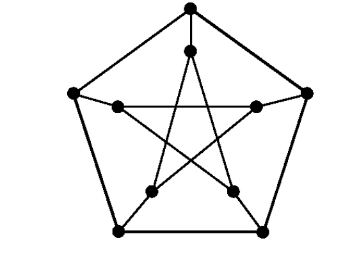
\includegraphics[width=0.2\columnwidth]{figs/q50.png}
\caption{Fig Question}
\label{fig:q50}
\end{figure}
\begin{enumerate}
\item The chromatic number of the graph is 3
\item The graph has a Hamiltonian path
\item The given graph is isomorphic to the Peterson graph
\begin{figure}[H]
\centering
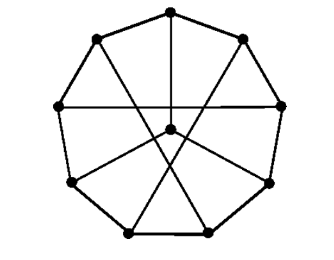
\includegraphics[width=0.2\columnwidth]{figs/q50-1.png}
\caption{Option 3}
\label{fig:q50}
\end{figure}
\item The size of the largest independent set of the given graph is 3
\end{enumerate}

\hfill{\brak{\text{GATE CS 2022}}}

\item Consider the following recurrence:  

$f(1)=1$  

$f(2n)=2f(n)+1, \quad n \geq 1$  

$f(2n+1)=2f(n)+1, \quad n \geq 1$  

Which of the following statements is/are TRUE?  

\begin{enumerate}
\item $f(2n-1)=2n-1$
\item $f(2n)=n$
\item $f(5 \cdot 2^n)=2n+1$
\item $f(2n+1)=2n+1$
\end{enumerate}

\hfill{\brak{\text{GATE CS 2022}}}

\item Which of the properties hold for the adjacency matrix $A$ of a simple undirected unweighted graph having $n$ vertices?  

\begin{enumerate}
\item The diagonal entries of $A^2$ are the degrees of the vertices of the graph
\item If the graph is connected, then none of the entries of $A^{n-1}+I_n$ can be zero
\item If the sum of all the elements of $A$ is at most $2(n-1)$, then the graph must be acyclic
\item If there is at least a 1 in each of $A$’s rows and columns, then the graph must be connected
\end{enumerate}

\hfill{\brak{\text{GATE CS 2022}}}

\item Which of the following is/are the eigenvector(s) for the matrix  

\[
\begin{bmatrix}
-9 & -6 & -2 & -4\\
-8 & -6 & -3 & -1\\
-20 & -15 & -8 & -5\\
-32 & -21 & -7 & -12
\end{bmatrix}
\]

\begin{enumerate}
\item $\begin{bmatrix}-1\\1\\0\\1\end{bmatrix}$
\item $\begin{bmatrix}1\\0\\1\\-1\end{bmatrix}$
\item $\begin{bmatrix}-1\\0\\2\\2\end{bmatrix}$
\item $\begin{bmatrix}0\\1\\-3\\0\end{bmatrix}$
\end{enumerate}

\hfill{\brak{\text{GATE CS 2022}}}

\item Consider a system with 2 KB direct mapped data cache with a block size of 64 bytes. The system has a physical address space of 64 KB and a word length of 16 bits. During the execution of a program, four data words P, Q, R, and S are accessed in that order 10 times (i.e., PQRSPQRS...). The addresses of the first bytes of P, Q, R, and S are 0xA248, 0xC28A, 0xCA8A, and 0xA262, respectively. Which of the following statements is/are TRUE with respect to the data cache?  

\begin{enumerate}
\item Every access to S is a hit
\item Once P is brought to the cache it is never evicted
\item At the end of the execution only R and S reside in the cache
\item Every access to R evicts Q from the cache
\end{enumerate}

\hfill{\brak{\text{GATE CS 2022}}}

\item Consider routing table of an organization’s router:  

\begin{tabular}{|c|c|c|}
\hline
Subnet Number & Subnet Mask & Next Hop \\
\hline
12.20.164.0 & 255.255.252.0 & R1 \\
12.20.170.0 & 255.255.254.0 & R2 \\
12.20.168.0 & 255.255.254.0 & Interface 0 \\
12.20.166.0 & 255.255.254.0 & Interface 1 \\
default &  & R3 \\
\hline
\end{tabular}


Which of the following prefixes in CIDR notation can be collectively used to correctly aggregate all of the subnets in the routing table?  

\begin{enumerate}
\begin{multicols}{2}
\item 12.20.164.0/20
\item 12.20.164.0/22
\item 12.20.164.0/21
\item 12.20.168.0/22
\end{multicols}
\end{enumerate}

\hfill{\brak{\text{GATE CS 2022}}}

\item Consider the relational database with the following four schemas and their respective instances:  

Student(sNo,sName,dNo), Dept(dNo,dName), Course(cNo,cName,dNo), Register(sNo,cNo)  
\begin{circuitikz}
\draw (0,0) node[xor port] (xor) {};
\draw (xor.in 1) to[short,-o] (-1,0.3) node[left] {$D_{in}$};
\draw (xor.in 2) to[short] (-1,-0.3) to (0,-0.3) node[flipflop] {};
\draw (xor.out) to[short,-o] (1,0) node[right] {$X$};
\end{circuitikz}

SQL Query:  

\begin{verbatim}
SELECT * FROM Student AS S WHERE NOT EXISTS
 (SELECT cNo FROM Course WHERE dNo="D01"
  EXCEPT
  SELECT cNo FROM Register WHERE sNo=S.sNo)
\end{verbatim}

The number of rows returned by the above SQL query is \rule{2cm}{0.4pt}  

\hfill{\brak{\text{GATE CS 2022}}}

\item Consider a network with three routers P, Q, R. All the links have cost unity. The routers exchange distance vector routing information and have converged on the routing tables, after which the link QR fails. Assume that P and Q send out routing updates at random times, each at the same average rate. The probability of a routing loop formation (rounded off to one decimal place) between P and Q, leading to count-to-infinity problem, is \rule{2cm}{0.4pt}  
\begin{figure}[H]
\centering
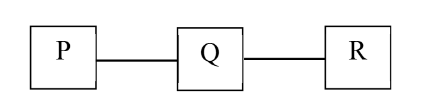
\includegraphics[width=0.8\columnwidth]{figs/q57.png}
\caption{Fig}
\label{fig:q57}
\end{figure}
\hfill{\brak{\text{GATE CS 2022}}}

\item Let $G(V,E)$ be a directed graph, where $V=\{1,2,3,4,5\}$. $A[i][j]=1$ for $1\leq j \leq i \leq 5$, 0 otherwise. The number of directed spanning trees rooted at vertex 5 is \rule{2cm}{0.4pt}  

\hfill{\brak{\text{GATE CS 2022}}}

\item Consider a 100 Mbps link between an earth station and a satellite at altitude 2100 km. Signal propagates at $3 \times 10^8$ m/s. The time taken (in ms, rounded off to two decimal places) for the receiver to completely receive a packet of 1000 bytes is \rule{2cm}{0.4pt}  

\hfill{\brak{\text{GATE CS 2022}}}

\item Consider TCP over a 1 Gbps link. Maximum segment lifetime (MSL) is 60 s. The minimum number of bits required for the sequence number field of the TCP header, to prevent wrapping around during the MSL, is \rule{2cm}{0.4pt}  

\hfill{\brak{\text{GATE CS 2022}}}

\item A processor X1 operating at 2 GHz has a standard 5-stage RISC pipeline with base CPI=1. For a program P with 30\% branches, control hazards incur 2-cycle stall for every branch. A new processor X2 at same frequency has branch predictor with 80\% accuracy, eliminating stalls for correctly predicted branches. The speedup (rounded off to two decimal places) obtained by X2 over X1 in executing P is \rule{2cm}{0.4pt}  

\hfill{\brak{\text{GATE CS 2022}}}

\item Consider queues $Q_1$ containing 4 elements and $Q_2$ empty. Only Enqueue and Dequeue allowed. The minimum number of Enqueue operations on $Q_1$ required to place elements of $Q_1$ into $Q_2$ in reverse order is \rule{2cm}{0.4pt}  
\begin{figure}[H]
\centering
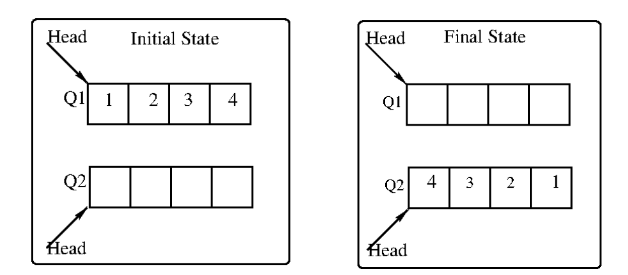
\includegraphics[width=0.8\columnwidth]{figs/q62.png}
\caption{Fig}
\label{fig:q62}
\end{figure}
\hfill{\brak{\text{GATE CS 2022}}}

\item Consider file systems A (contiguous allocation) and B (linked allocation). A file of 100 blocks is stored in both. Insert a new block between 50th and 51st. Let required disk accesses be $n_A$ and $n_B$. Then $n_A+n_B=$\rule{2cm}{0.4pt}  

\hfill{\brak{\text{GATE CS 2022}}}

\item Consider demand paging system with 4 page frames (initially empty) and LRU policy. For page reference string 7,2,7,3,2,5,3,4,6,7,7,1,5,6,1 the page fault rate (rounded off to one decimal place) is \rule{2cm}{0.4pt}  

\hfill{\brak{\text{GATE CS 2022}}}

\item Consider grammar with translation rules:  

$S \to S_1 \# T \quad \{S.val = S_1.val * T.val\}$  

$S \to T \quad \{S.val = T.val\}$  

$T \to T_1 \% R \quad \{T.val = T_1.val / R.val\}$  

$T \to R \quad \{T.val = R.val\}$  

$R \to id \quad \{R.val = id.val\}$  

For the expression $20\#10\%5\#8\%2\%2$, the computed value of $S.val$ is \rule{2cm}{0.4pt}  

\hfill{\brak{\text{GATE CS 2022}}}
\begin{table}[h!]
\centering
\begin{tabular}{|c|c|c|c|c|c|}
\hline
Q. No. & Session & Question Type & Subject Name & Key/Range & Mark \\
\hline
1  & 1 & MCQ & GA & D & 1 \\
2  & 1 & MCQ & GA & C & 1 \\
3  & 1 & MCQ & GA & D & 1 \\
4  & 1 & MSQ & GA & A,B,D & 2 \\
5  & 1 & NAT & GA & 26.50 to 26.50 & 1 \\
6  & 1 & MCQ & GA & A & 1 \\
7  & 1 & NAT & GA & 9.00 to 9.00 & 1 \\
8  & 1 & MCQ & GA & B & 1 \\
9  & 1 & MCQ & GA & D & 1 \\
10 & 1 & NAT & GA & 21.00 to 21.00 & 1 \\
11 & 1 & MCQ & CS & B & 1 \\
12 & 1 & MCQ & CS & C & 1 \\
13 & 1 & MCQ & CS & B & 1 \\
14 & 1 & NAT & CS & 16.00 to 16.00 & 1 \\
15 & 1 & MCQ & CS & C & 1 \\
16 & 1 & MCQ & CS & C & 1 \\
17 & 1 & MCQ & CS & A & 1 \\
18 & 1 & MCQ & CS & B & 1 \\
19 & 1 & MCQ & CS & D & 1 \\
20 & 1 & MCQ & CS & C & 1 \\
21 & 1 & MCQ & CS & C & 2 \\
22 & 1 & MCQ & CS & D & 2 \\
23 & 1 & MCQ & CS & C & 2 \\
24 & 1 & MCQ & CS & B & 2 \\
25 & 1 & MSQ & CS & A,B,D & 2 \\
26 & 1 & MCQ & CS & A & 2 \\
27 & 1 & MCQ & CS & C & 2 \\
28 & 1 & MSQ & CS & A,C & 2 \\
29 & 1 & MCQ & CS & A & 2 \\
30 & 1 & MCQ & CS & B & 2 \\
31 & 1 & MCQ & CS & D & 2 \\
32 & 1 & MCQ & CS & A & 2 \\
33 & 1 & MCQ & CS & B & 2 \\
34 & 1 & MCQ & CS & D & 2 \\
35 & 1 & MCQ & CS & A & 2 \\
36 & 1 & MCQ & CS & D & 2 \\
37 & 1 & MCQ & CS & D & 2 \\
38 & 1 & MCQ & CS & A & 2 \\
39 & 1 & MCQ & CS & A & 2 \\
40 & 1 & MCQ & CS & D & 2 \\
41 & 1 & MCQ & CS & A & 2 \\
42 & 1 & MCQ & CS & B & 2 \\
43 & 1 & MCQ & CS & C & 2 \\
44 & 1 & MCQ & CS & A & 2 \\
45 & 1 & MCQ & CS & B & 2 \\
46 & 1 & MSQ & CS & A,B,C & 2 \\
47 & 1 & MSQ & CS & B,C & 2 \\
48 & 1 & MSQ & CS & A,C,D & 2 \\
49 & 1 & MSQ & CS & C,D & 2 \\
50 & 1 & MSQ & CS & A,B,C & 2 \\
51 & 1 & MSQ & CS & A,B,C & 2 \\
52 & 1 & MSQ & CS & A,B,C & 2 \\
53 & 1 & MCQ & CS & B & 2 \\
54 & 1 & MSQ & CS & A,B,C & 2 \\
55 & 1 & MCQ & CS & B & 2 \\
56 & 1 & NAT & CS & 2.00 to 2.00 & 2 \\
57 & 1 & NAT & CS & 0.50 to 0.50 & 2 \\
58 & 1 & NAT & CS & 24.00 to 24.00 & 2 \\
59 & 1 & NAT & CS & 8.00 to 8.00 & 2 \\
60 & 1 & NAT & CS & 31.00 to 31.00 & 2 \\
61 & 1 & NAT & CS & 1.13 to 1.13 & 2 \\
62 & 1 & NAT & CS & 6.00 to 6.00 & 2 \\
63 & 1 & NAT & CS & 1.00 to 1.00 & 2 \\
64 & 1 & NAT & CS & 7.00 to 7.00 & 2 \\
65 & 1 & NAT & CS & 80.00 to 80.00 & 2 \\
\hline
\end{tabular}
\caption*{}
\label{tab:answerkey}
\end{table}



\end{enumerate}
\end{document}